% thesis.tex -- 論文の書き方参考例
%
% (注意)氏名、学籍番号等を変更すること。
%
% (LaTeXの実行法) platex thesis.tex
%
%	このファイル内にある '% 'はコメント。
%
\documentclass[a4j,11pt]{jreport}
\usepackage{ascmac}
\usepackage{amsmath}
\usepackage{float}
\usepackage{url}
\usepackage[dvipdfmx]{graphicx}
\usepackage{thesis-master}
\usepackage{mylatex}
\pagestyle{plain}

% 所属研究科、専攻
\courseofmastercs
% 研究テーマ
\title{ヒルベルト-ファン変換を適用したゴルフスイング解析}
% 氏名
\author{木~~村~~~勇~~大}
% 学籍番号
\id{G~~2~~1~~2~~1~~0~~2~~1}
% 指導教員
\teacher{生~野~~壮~一~郎}
% 提出日
\date{20XX}{X}{X}
% 提出年度
\schoolyear{2022}

% 研究室名(カバー用)
\clab{生野}
% 学籍番号(カバー用)
\cid{G2121021}

%% 英語要旨
\etitle{Numerical Analysis of Golf Swing using Hilbert-Huang Transformation}
\eauthor{Y~u~d~a~i~~K~i~m~u~r~a}
\eteacher{S~o~i~c~h~i~r~o~~I~k~u~n~o}

\begin{document}
%\makecover		% カバー(提出電子化に伴い削除)
\maketitle		% 表紙

% 修士論文和文要旨
\jabst{
% abstract.tex -- 論文概要
修士論文の概要を記述.
	% 00jabstract.texを読み込む
}
\makejabstract

% 修士論文英文概要
\eabst{
% abstract.tex -- 論文概要
Write an abstract of your Paper.

}
\makeeabstract

% 目次
\pagenumbering{roman}
\setcounter{page}{1}
\thispagestyle{plain}
\tableofcontents	% 目次
\listoffigures		% 図目次
\listoftables		% 表目次
%\listofprograms		% プログラム目次

% 論文本文
%   論文本文は章や節単位で,いくつかのファイルに分割したほうが編集しやすい.
% \input{hogehoge}	% hogehoge.texを読み込む.
% 章構成は適宜変更すること.
\pagenumbering{arabic}
\chapter{例: 序論}
\section{はじめに}
\section{研究目的}		% 第1章 序論
\chapter{ヒルベルト・ファン変換}
%
ヒルベルト・ファン変換(HHT : Hilbert Huang Transform)とは,
信号$x(t)$ を,経験的モード分解(EMD : Empirical Mode Decomposition)より,有限の固有モード関数(IMF : Intrinsic Mode Function)$\sum_{k=1}^{n}{\rm{IMF}}_{k}$ と一つの残差に分解し,
分解した${\rm{IMF}}_{k}$ にヒルベルト変換を適用させ,瞬時周波数$\omega(t)$ と瞬時振幅$A(t)$ を求める手法である.
%

% 瞬時周波数$\omega(t)$ と瞬時振幅$A(t)$の求め方は,解析信号$z(t) = z_{r}(t) + iz_{i}(t)$の実部$z_{r}(t)$ と虚部$z_{i}(t)$から以下の式のように求める.
% \begin{equation}
%     \label{inst freq}
%     \omega(t) = \frac{d}{dt}\arctan\frac{z_{i}(t)}{z_{r}(t)}
% \end{equation}

% \begin{equation}
%     \label{inst amp}
%     A(t) = |z(t)|
% \end{equation}

% また,解析信号の虚部である$z_{i}(t)$ を求めるために,実部$z_{r}(t)$ を経験的モード分解より得られた$\sum_{k=1}^{n}{\rm{IMF}}_{k}$ とし,その実部$z_{r}(t)$にヒルベルト変換を適用させることで,虚部$z_{i}(t)$ を求めることができる.
% 以下は,$z_{r}(t) = \sum_{k=1}^{n}{\rm{IMF}}_{k}$ にヒルベルト変換を適用させた式である.$\rm{PV}$ は,コーシーの主値である.
% \begin{equation}
%     z_{i}(t) = \frac{1}{\pi}PV \int_{-\infty}^{\infty} \frac{z_{r}(t)}{t - \tau} d \tau = \frac{1}{\pi t} * z_{r}(t)
% \end{equation}
% 次節からは,HHTで使用されているEMDのアルゴリズム,多変量に拡張された多変量経験的モード分解について説明する.
%
%=================================================================================================================================================================================================================================%
\section{EMD}
%
EMDとは,信号$x(t)$ が有限の固有モード関数$\rm{IMF}_{k}$ と残差$r(t)$ で構成されていると仮定し,ヒューリスティックに分解する.
EMDの式を以下で示す.
\begin{equation}
    \label{emd}
    x(t) = \sum_{k=1}^{n} {\rm{IMF}}_{k} + r(t)
\end{equation}

${\rm{IMF}}_{k}$ は,以下の2つの条件を満たす.
\begin{itemize}
    \item 局所的極値の数とゼロ交差の数が0,または1であること.
    \item 局所的極値から構成された上側包絡線と下側包絡線の平均値が0であること.
\end{itemize}
%
EMDのアルゴリズムを以下に示す.
\begin{enumerate}
    \item 残差を計算.($r(t) = x(t)$ とする.)
    \begin{equation}
        r(t) = \sum_{k=1}^{n} {\rm{IMF}}_{k} - x(t)
    \end{equation}
    \item ${\rm{IMF}}_{\rm{old}}(t) = r(t)$ と初期化して,${\rm{IMF}}_{k}$を取り出す.
    \begin{enumerate}
        \item ${\rm{IMF}}_{\rm{old}}(t)$ の極大値を結ぶ包絡線$u(t)$ と,極小値を結ぶ包絡線$l(t)$ を三次スプライン補完で求め,$u(t)$ と$l(t)$ の平均を${\rm{IMF}}_{\rm{old}}(t)$ から引く.
        \begin{equation}
            {\rm{IMF}}_{\rm{new}}(t) = {\rm{IMF}}_{\rm{old}}(t) - \frac{u(t) - l(t)}{2}
        \end{equation}
        \item ${\rm{IMF}}_{\rm{new}}(t)$ が収束条件SD$(0.2 \leq SD \leq 0.3)$ を満たす場合,${\rm{IMF}}$ 集合に追加し,満たさない場合は(a),(b)を繰り返す.SDの収束条件は以下の式である.
        \begin{equation}
            SD = \sum_{t=1}^{n} \frac{({\rm{IMF}}_{\rm{old}}(t) - {\rm{IMF}}_{\rm{new}}(t) )^2}{{\rm{IMF}}_{\rm{new}}(t)^2 }
        \end{equation}
        
    \end{enumerate}
    \item $\sum_{k=1}^{n} {\rm{IMF}}_{k}$ が全て取り出されるまで,1,2を繰り返す.
\end{enumerate}

%
%=================================================================================================================================================================================================================================%
\section{多変量経験的モード分解}
%
一般に,多チャンネルに拡張された経験的モード分解として,多変量経験的モード分解(MEMD : Multivariate EMD)が提案されている.
本研究では,複数のセンサからヒトの動作を採取するため,MEMDを採用する.
%
%=================================================================================================================================================================================================================================%
\section{解析信号}
%
解析信号は,実信号が負の周波数成分を持たない信号として定義される.
以下に,解析信号の式を示す.%参考文献チェック
\begin{equation}
    \label{analyse signal}
    z(t) = z_{r}(t) + iz_{i}(t)
\end{equation}
本節では,解析信号の導出について説明する.

実信号$z_{r}(t) = x(t)$のスペクトル$X(\omega)$とし,$x(t)$と$X(\omega)$を以下の式で表現する.
\begin{equation}
    \label{x(t)}
    x(t) = \frac{1}{\sqrt{2\pi}} \int X(\omega) e^{i \omega t} d\omega
\end{equation}
%
\begin{equation}
    \label{X(t)}
    X(\omega) = \frac{1}{\sqrt{2\pi}} \int x(t) e^{-i\omega t} dt
\end{equation}
%
複素信号$z(t)$は,スペクトル$X(t)$のせいの周波数成分のみからなることから,次の式のように,$X(t)$の正の周波数部分のフーリエ逆変換として得られる.
\begin{equation}
    \label{iF(t)}
    z(t) = 2 \frac{1}{\sqrt{2\pi}} \int_{0}^{\infty} X(\omega) e^{i\omega t} d\omega
\end{equation}
%
\ref{iF(t)}式の係数$2$は,解析信号の実部を$x(t)$と等しくするためのものである.
よって,\ref{X(t)}式を用いると\ref{iF(t)}式は,
%
\begin{eqnarray}
    z(t) &=& 2 \frac{1}{2\pi} \int_{0}^{\infty} \int x(t^{\prime}) e^{-i\omega t^{\prime}} e^{i\omega t} dt^{\prime} d\omega \\
         &=& \frac{1}{\pi} \int_{0}^{\infty} \int x(t^{\prime}) e^{i\omega (t - t^{\prime})} dt^{\prime} d\omega \label{z(t)変換途中1}
\end{eqnarray}
%
% ここで,デルタ関数$\int_{0}^{\infty} e^{j\omega x} d\omega = \pi \delta (x) + \frac{j}{x}$より,
ここで,ステップ関数$u(\omega)$のフーリエ変換式は以下の式である.
\begin{equation}
    \label{ft step function}
    \int_{0}^{\infty} u(\omega) e^{i \omega x} = \pi \delta (x) + \frac{i}{x}
\end{equation}
%
\ref{ft step function}式を用いると,\ref{z(t)変換途中1}式は,
\begin{equation}
    z(t) = \frac{1}{\pi} \int x(t^{\prime}) \biggl[ \pi \delta (t - t^{\prime}) + \frac{i}{t - t^{\prime}} \biggr] dt^{\prime}
\end{equation}
%
となるため,結果以下の式のように解析信号が導出される.
\begin{equation}
    \label{解析信号オリジナル}
    z(t) = x(t) + \frac{i}{\pi} \int \frac{x(t^{\prime})}{t - t^{\prime}} dt^{\prime}
\end{equation}
%
ここで,$x(t) = z_{r}(t)$に戻し,\ref{解析信号オリジナル}式の第2項を$z_{i}(t)$とおくと,$z_{i}(t)$は以下の式のように表現することができる.
\begin{equation}
    \label{ヒルベルト変換}
    z_{i}(t) = H[z_{r}(t)] = \frac{1}{\pi} \int \frac{x(t^{\prime})}{t - t^{\prime}} dt^{\prime}
\end{equation}
%
%=================================================================================================================================================================================================================================%
\section{ヒルベルト変換}
%参考文献チェック
前節では,解析信号の導出について説明したが,その虚部$z_{i}(t)$は,\ref{ヒルベルト変換}式よりヒルベルト変換で求められることを示した.
ヒルベルト変換とは,与えられた関数の周波数成分の位相を$-\frac{\pi}{2}$ずらす操作である.
以下は,信号$x(t)$のスペクトルを$X(t)$とした時のヒルベルト変換式の導出を示す.

実信号$x(t) =\cos (\omega t)$と直交する虚部は,
\begin{equation}
    \label{cosから90度位相を遅らせた式}
    \cos (\omega t - \frac{\pi}{2}) =\sin (\omega t)
\end{equation}
である.
%
よって,実部$\cos (\omega t + \phi)$,虚部を\ref{cosから90度位相を遅らせた式}式より$\sin (\omega t + \phi)$とし,複素指数関数を立式すると以下の式のようになる.
\begin{equation}
    \label{複素指数関数}
    e^{i(\omega t + \phi)} = \cos (\omega t + \phi) + i \sin(\omega t + \phi)
\end{equation}
\ref{複素指数関数}式に,虚数単位$-i$を1回かけると
\begin{equation}
    \label{-i1回目}
    -i e^{i(\omega t + \phi)} = -i \cos (\omega t + \phi) + \sin(\omega t + \phi)
\end{equation}
となる.
この時の実部は$\sin(\omega t + \phi)$となり,\ref{複素指数関数}式の実部より$\frac{\pi}{2}$遅れていることが確認できる.
%
さらに,\ref{-i1回目}式に$-i$をかけると,
\begin{equation}
    -e^{i(\omega t + \phi)} = -\cos(\omega t + \phi) - i \sin(\omega t + \phi)
\end{equation}
となり,実部に注目すると\ref{-i1回目}式の実部より,位相が$\frac{\pi}{2}$遅れていることが確認できる.
%
\begin{equation}
    -\cos(\omega t + \phi) = \sin(\omega t + \phi - \frac{\pi}{2})
\end{equation}
%
すなわち,虚数単位$i$をかけることで,$\frac{\pi}{2}$位相を遅らせることができる.
しかしながら,これは連続された関数のみに適応が可能であるため,離散的関数の位相を$\frac{\pi}{2}$遅らせるには,$-i {\rm{sgn}}(f)$をかける必要がある.
%

実信号$x(t)$のスペクトルを$X(t)$とする時,全ての周波数成分の位相を$\frac{\pi}{2}$遅らせるには,スペクトル$X(t)$に$-i {\rm{sgn}} (f)$をかけ,その結果をフーリエ逆変換する必要がある.
まず,$X(f)$に$-i{\rm{sgn}}(f)$を掛けた直行スペクトルを$X_{\perp}(t)$とすると,以下の式のように表現できる.
\begin{equation}
    \label{X(t)の直行スペクトル}
    X_{\perp}(f) = -i {\rm{sgn}} (f) X (f)
\end{equation}
%
次に,\ref{X(t)の直行スペクトル}式より,$X_{\perp} (f)$のフーリエ逆変換を行うことで,$x(t)$の直行スペクトル$x_{\perp}(t)$を得ることができる.
以下は,$x_{\perp}(t)$の式である.
\begin{equation}
    \label{x(t)垂直}
    x_{\perp} (t) = -i \int^{+\infty}_{-\infty} {\rm{sgn}} (f) X(f) e^{2 i \pi f t} df
\end{equation}
%
ここで,$-i {\rm{sgn}} (f)$のフーリエ逆変換は以下の式である.
\begin{equation}
    \label{シグナル関数のフーリエ変換}
    F^{-1} \lbrace -i {\rm{sgn}} (f) \rbrace = \frac{1}{\pi t}
\end{equation}
%
そして,$X(f)$のフーリエ逆変換は$x(t)$である.
よって,\ref{x(t)垂直}式は,以下の式のように書くことができる.
\begin{equation}
    \label{ヒルベルト変換}
    x {\perp} (t) = \frac{1}{\pi} \int^{+\infty}_{-\infty} \frac{1}{t - \tau} x(\tau) d\tau
\end{equation}
%
一般に\ref{ヒルベルト変換}式は,ヒルベルト変換の公式と言われている.

%		% 第2章 関連技術
\chapter{ゴルフスイングのバイオメカニズム}
%=================================================================================================================================================================================================================================%
\section{バイオメカニクス}
%
バイオメカニクス(biomechanics)とは,生体に力が作用して起こる現象を取り扱う,力学の一分野であり,日本語では生体力学,あるいは生体機械工学とも呼ばれる.
バイオメカニクスでは,ヒトをはじめとする全生物を対象とし,対象の生物の器官系,器官,組織,細胞,遺伝子といった,各レベルまで扱う.
バイオメカニクスの歴史として,14世紀から16世紀に急速にヒトの内部の仕組みを知りたいという願望が増大し,その中でも,レオナルド・ダ・ビンチが人体解剖図を精密化したことが有名である.

現在のバイオメカニクスは,バイオメカニクスと関連した学問や分野が発展し,解剖学,生理学,医用工学,人間工学,スポーツ工学といった分野がよく関連されている.

%=================================================================================================================================================================================================================================%
\section{人体構造}
図\ref{基本的立位姿勢}は基本的立位姿勢を示す.
\begin{figure}
    \begin{center}
        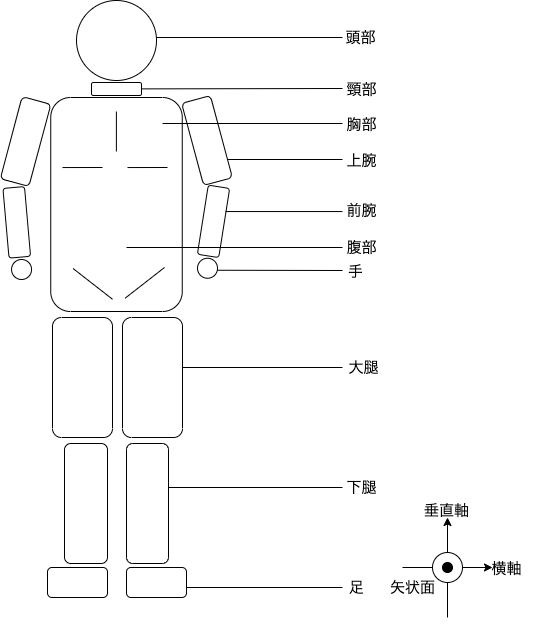
\includegraphics[width=1.0\linewidth]{./images/human_body.png}
        \caption{基本的立位姿勢}
        \label{基本的立位姿勢}
    \end{center}
\end{figure}
ヒトには,いくつかの部位のグループで呼ばれることがある.
一般に体幹と呼ばれるグループがあるが,
広い幅の意味を持つ体幹とは図\ref{基本的立位姿勢}より,頭部,頸部,胸部,腹部のグループであり,その中でも胸部,腹部のみでも体幹と呼ばれることがある.
上腕,前腕,手の三部位を総称し上肢と呼び,大腿,下腿,足の三部位を総称し下肢と呼ぶ.
また,上肢,下肢を総称し体肢,四肢と呼ばれることがある.
% 本研究もこの名称に従い,部位の名称を扱う.

次に,運動の基準とする軸について説明する.
図\ref{基本的立位姿勢}より,床と頭部を結ぶ軸を垂直軸,床と左右に並行の軸を横軸,背面から前方方向への軸を矢状軸と呼ぶ.


% \section{関節}
% 本節ではヒトの関節名称を示す.
% \begin{figure}
%     \begin{center}
%         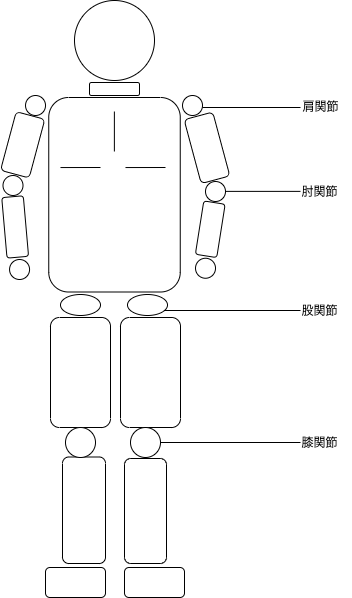
\includegraphics[width = 5cm]{./images/joint.png}
%         \caption{関節構造}
%         \label{関節構造}
%     \end{center}
% \end{figure}
% 図\ref{関節構造}の,

%=================================================================================================================================================================================================================================%
\section{人体の運動表現}
ヒトが運動する際に,その時の運動の表現は世界共通の表現がある.
本節では,日本整形外科学会の規則に則り,ヒトの運動表現について説明する.

ヒトには,屈曲/伸展,外転/内転,外旋/内旋の三種類の基本動作がある.
屈曲/伸展とは,横軸に並行な運動である.
一般に,頭部,胸部が前方に倒れる方向を屈曲,反対の動きを伸展と呼ぶ.
外転/内転とは,矢状軸に並行な運動である.
一般に,上肢を床と並行,矢状軸と直角になる運動を外転,反対の動きを内転と呼ぶ.
また,頸部,胸部,腰部は定義に則した運動に一致しないことから,側屈と呼ばれることがある.
外旋/内旋とは,垂直軸に並行な運動である.
一般に,前腕を床と並行かつ上腕と直角にした状態で,上体の方向に回転する運動を内旋,上体から離れるような回転を外旋と呼ぶ.
また,頸部,胸部,腰部は定義則した運動に一致しないことから,回旋や捻転と呼ばれることがある.

%=================================================================================================================================================================================================================================%
\section{ゴルフ}
%
現在,日本のゴルフはかなり盛んであり,プロゴルファーの松山や渋野が海外で活躍するのをきっかけに,全世代的に見ても流行の兆しがある.
特に,日本のゴルフ用品の市場規模は,世界二位の2000億円であり,ますます期待されるスポーツである.

ゴルフの初心者等は,上達のためにスクールに通いインストラクターをつけ,最新の器具や設備,解析機器を使用して練習に励む動向がある.
特に現代の技術では,
ハイスピードカメラや高性能カメラを使用したモーションキャプチャを用いたゴルフスイング解析,
トラックマンを使用したゴルフボールの弾道測定,
また,動画技術も向上したため様々な流儀のスイング解説がある.

ゴルフとは,最小打数でボールをカップに入れること競うスポーツである.
ゴルフをプレーするにあたり,フィールドが用意されているが,ゴルフでは打ち初めからカップに入れるまでにプレーを行うフィールドをホールと呼ぶ.
各ホールには規定打数が決められており,3打数(パー3)が4ホール,4打数(パー4)が10ホール,5打数(パー5)が4ホールの計18ホール(1ラウンド)があり,1ラウンドを規定打数通りにプレーすると72打数で終了することとなる.

各ホールには,5つのエリアが定義されている.
5つのエリアとは,
プレイヤーが必ず打ち始めを行うティーイングエリア,
フェアウェイ,ラフ,その他の自然物を含めたジェネラルエリア,
プレイヤーの能力をテストするために特別に設置されたバンカーエリア,
ボールを地面で転がしカップに入れること目的としたパッティンググリーン,
そして,主にプレーを続行することが不能となりペナルティーが課せられるペナルティーエリアがある.

ゴルフの競技性として,規定打数より少ない打数でカップに入れられたプレイヤーが勝利となるため,プレイヤーは,ティーイングエリアからスタートしパッティンググリーンのカップへ効率良くいれることが必要である.
故に,バンカーエリアやペナルティーエリアをさけ,可能な限りジェネラルエリア,特にフェアウェイ上でプレイされることが望ましい.

%=================================================================================================================================================================================================================================%
\section{ゴルフボールの弾道}
ゴルフの基本として,真っ直ぐかつ遠くに飛ばすことが理想である.
しかしながら,一般ゴルファーにとってストレート弾道に飛球させることはかなり難しい.
特に,一般ゴルファーに起こりやすいミスとしてよく挙げられることは,右に曲がるスライス弾道や,左に曲がってしまうフック弾道がある.

スライス弾道となるメカニズムは,クラブフェースがボールに対し右向きでヒットすることにより,ボールの回転が右回転するためである.
クラブフェースが右向きでボールにヒットすることを,オープンフェースと呼ばれるが,オープンフェースの主な原因は,クラブの軌道がインサイドアウトになってしまうことである.
フック弾道となるメカニズムは,クラブフェースがボールに対し左向きでヒットすることにより,ボールの回転が左向きになるためである.
クラブフェースが左向きでボールにヒットすることを,クローズフェースと呼ばれるが,クローズフェースの主な原因は,クラブの軌道がアウトサイドインになってしまうことである.
すなわち,ゴルフボールを真っ直ぐに飛ばすためには,クラブフェースがボールに対し並行(スクエアフェース)でヒットすることが重要であり,これを実現するためには,クラブがインサイドインの軌道を描くことが需要である.

一般ゴルファーや初心者ゴルファーは,スライス弾道になってしまうことがよくあるが,その原因としてヘッドアップ動作や身体が開く動作が原因として上がる.
次節にて,ヘッドアップ動作,身体が開く動作について説明する.

%=================================================================================================================================================================================================================================%
\section{ヘッドアップ動作と身体が開く動作}
前節にて,一般ゴルファーや初心者ゴルファーにはヘッドアップ動作や身体が開く動作がよく起こると述べた.

\begin{figure}
    \begin{center}
        \begin{tabular}{c}
            \begin{minipage}{0.5\hsize}
                \begin{center}
                    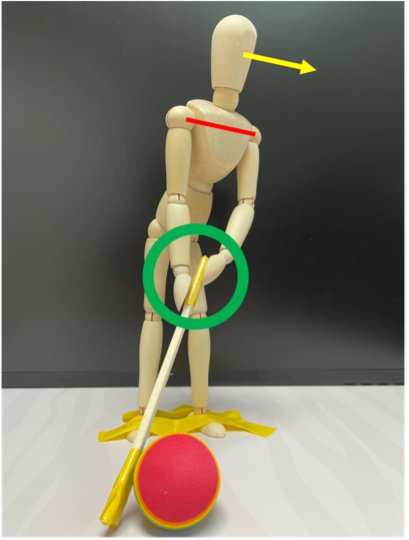
\includegraphics{./images/headup.png}
                    \caption{ヘッドアップ動作}
                    \label{headup}
                \end{center}
            \end{minipage}

            \begin{minipage}{0.5\hsize}
                \begin{center}
                    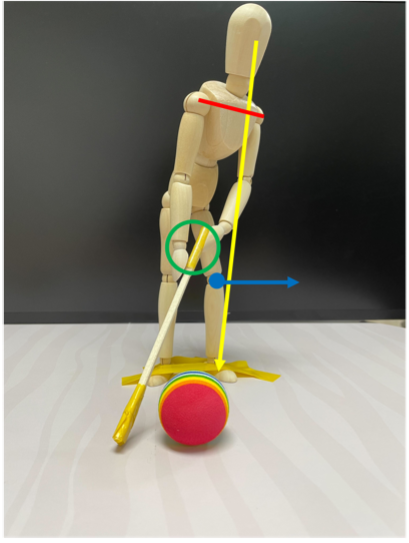
\includegraphics{./images/opening.png}
                    \caption{身体が開く動作}
                    \label{opening}
                \end{center}
            \end{minipage}
        \end{tabular}
    \end{center}
\end{figure}

ヘッドアップ動作とは,\ref{headup}の黄色線のように目線がインパクトする前に打球方向へ頸部が回旋動作である.
また,アドレス時の前傾姿勢をインパクト時まで保てずに頭部が伸展する動作もヘッドアップに分類される.
この動作により,図1の赤線のようにインパクト前に上半身が伸展\ref{headup}の緑円ように腕が振り遅れるため,
クラブフェースがオープンフェースへ誘起され,結果としてスライス弾道が起こる.

身体の開きの動作とは,\ref{opening}の赤線や青線のようにヒトの正面胸部や前足軸の膝がインパクトより前に打球方向へ外旋動作である.
この動作もヘッドアップ動作同様で,図2の緑円のように上体より腕が振り遅れてしまうため,クラブフェースがオープンフェースへ誘起される.

ヘッドアップ動作やインパクト前の身体の開きは,スイングを撮影した動画を見ただけでは初心者やアベレージゴルファーにとっては,特定するのは非常に困難であることが知られている.
また,その動作がどの部位にどのタイミングで起こっていることを特定することは非常に困難である.
そこで,本研究では特にスライス弾道の原因となるヘッドアップ動作とインパクト前の身体の開き動作に焦点をあて,頭部と身体の開き関係する関節部に注目してスイングの解析を行う.
本研究は,スライス弾道の大きな原因と言われるヘッドアップ動作,身体の開きの動作より,頭部と身体の開き関係する関節部に注目して解析を行う.	% 第3章 提案
\chapter{解析結果}
本研究は,ゴルフスイングを数値化したデータに,ヒルベルト・ファン変換を適用させ,瞬時周波数領域で解析を行う.
\section{ゴルフスイングの数値化}
ゴルフスイングの数値化は,慣性式モーションキャプチャを使用して行う.
使用するモーションキャプチャは,PERCEPTION NEURON 2.0を使用する.
\begin{figure}
    \begin{center}
        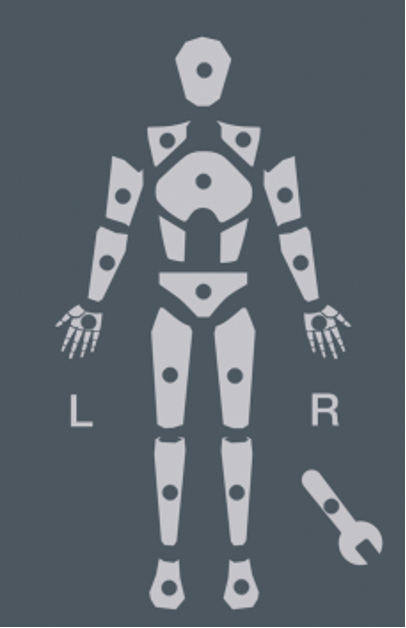
\includegraphics[width=3.5cm]{./images/sensors.png}
        \caption{加速度センサがついている位置}
        \label{sensors}
    \end{center}
\end{figure}
PERCEPTION NEURON 2.0は,図\ref{sensors}のように17点の位置に加速度センサを装着する.
この加速度センサより,推定の位置座標と$x$,$y$,$z$軸方向の回転角度を時系列にキャプチャしrawデータに書き出す.

PERCEPTION NEURON 2.0より,ゴルフスイングの時系列データを採取したrawデータであるため,bvh(biovision hierarchy)ファイルに変換する必要がある.
\begin{figure}
    \begin{center}
        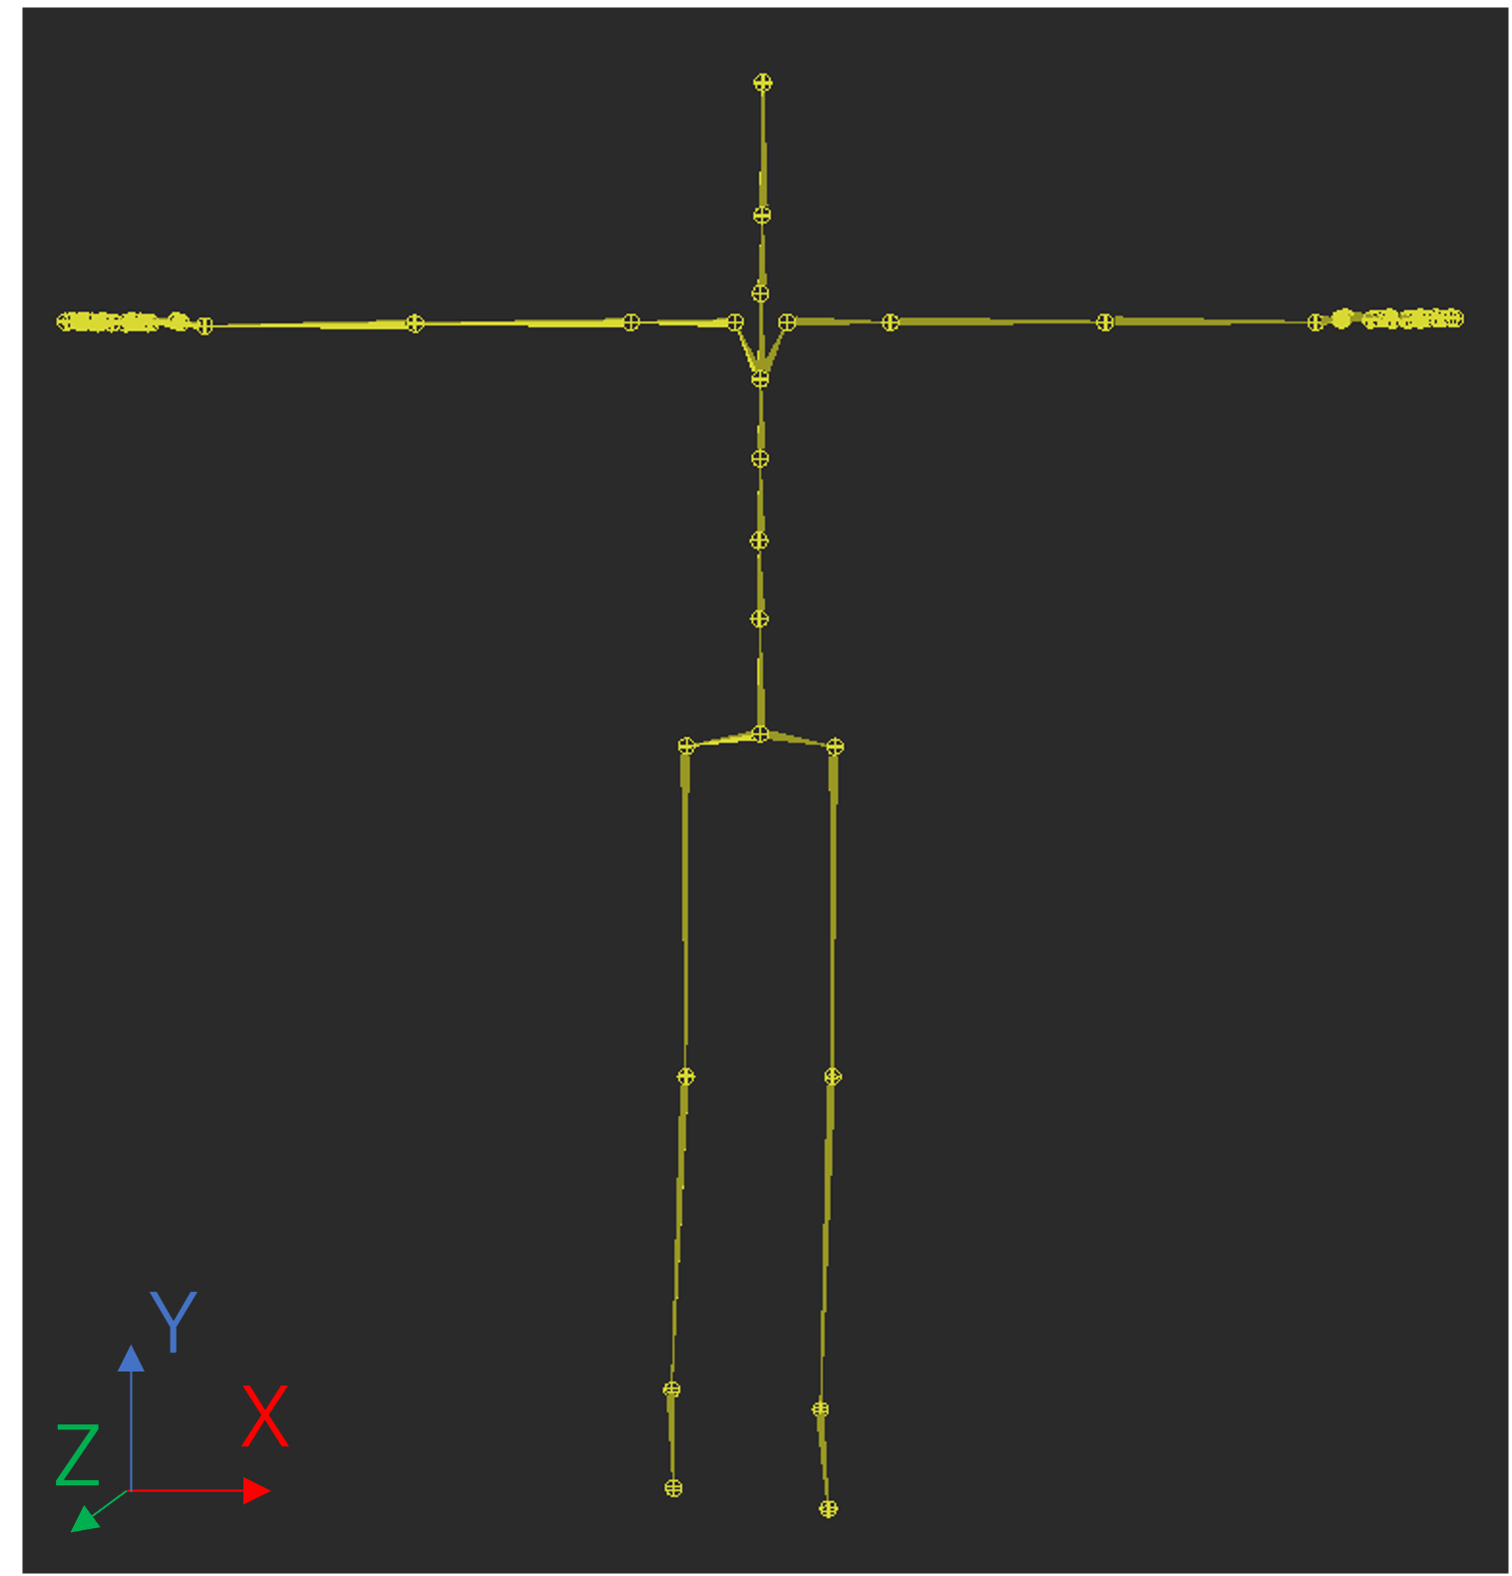
\includegraphics[width=5cm]{./images/Tpose.png}
        \caption{T-pose}
        \label{tpose}
    \end{center}
\end{figure}
bvhファイルとは,図\ref{tpose}のように指定された点の推定の位置座標や$x$,$y$,$z$軸方向の回転角を時系列に書き出したファイルである.
rawデータからbvhファイルの変換は,PERCEPTION NEURON 2.0専用ソフトであるAxis Neuronより行う.

図\ref{tpose}は,T-poseと呼ばれる,デフォルトポーズである.
このポーズより$x$,$y$,$z$軸方向を定義し,各関節球の$x$,$y$,$z$軸の回転角を0度とする.
bvhファイルに書き込まれている時系列データは,このポーズからの回転角を示し,ルートである腰部は$x$,$y$,$z$方向の位置座標も記録する.
よって,各関節球の3軸方向の回転角と腰部の3軸方向の位置座標を合計し,180チャンネルの時系列データを扱う.

\section{被験者情報}
被験者は,ゴルフ歴10年,平均スコア100のアベレージゴルファーである.
被験者にドライバーショットを行わせたところ,ストレート弾道に飛球したゴルフスイング,スライス弾道でヘッドアップ動作をしたゴルフスイング,スライス弾道で身体が開く動作をしたゴルフスイングの3種類採取することができ,各種類で6スイングずつデータを採取することができた.
本研究では,各スイングごとにヒルベルト・ファン変換を行い,瞬時周波数と瞬時振幅を求め,各種類毎に瞬時周波数の平均化,瞬時振幅平滑化を行う.

本研究では,アベレージゴルファーのスライスの原因としてよく挙げられるヘッドアップ動作,身体が開く動作をしたゴルフスイングに注目し,ストレート弾道に飛球したゴルフスイングと比較して考察を行う.

\section{スペクトログラム解析}
\subsection{頸部,左膝モーションのIMF1}
\begin{figure}
    \begin{center}
        \begin{tabular}{c}
            \begin{minipage}{0.5\hsize}
                \begin{center}
                    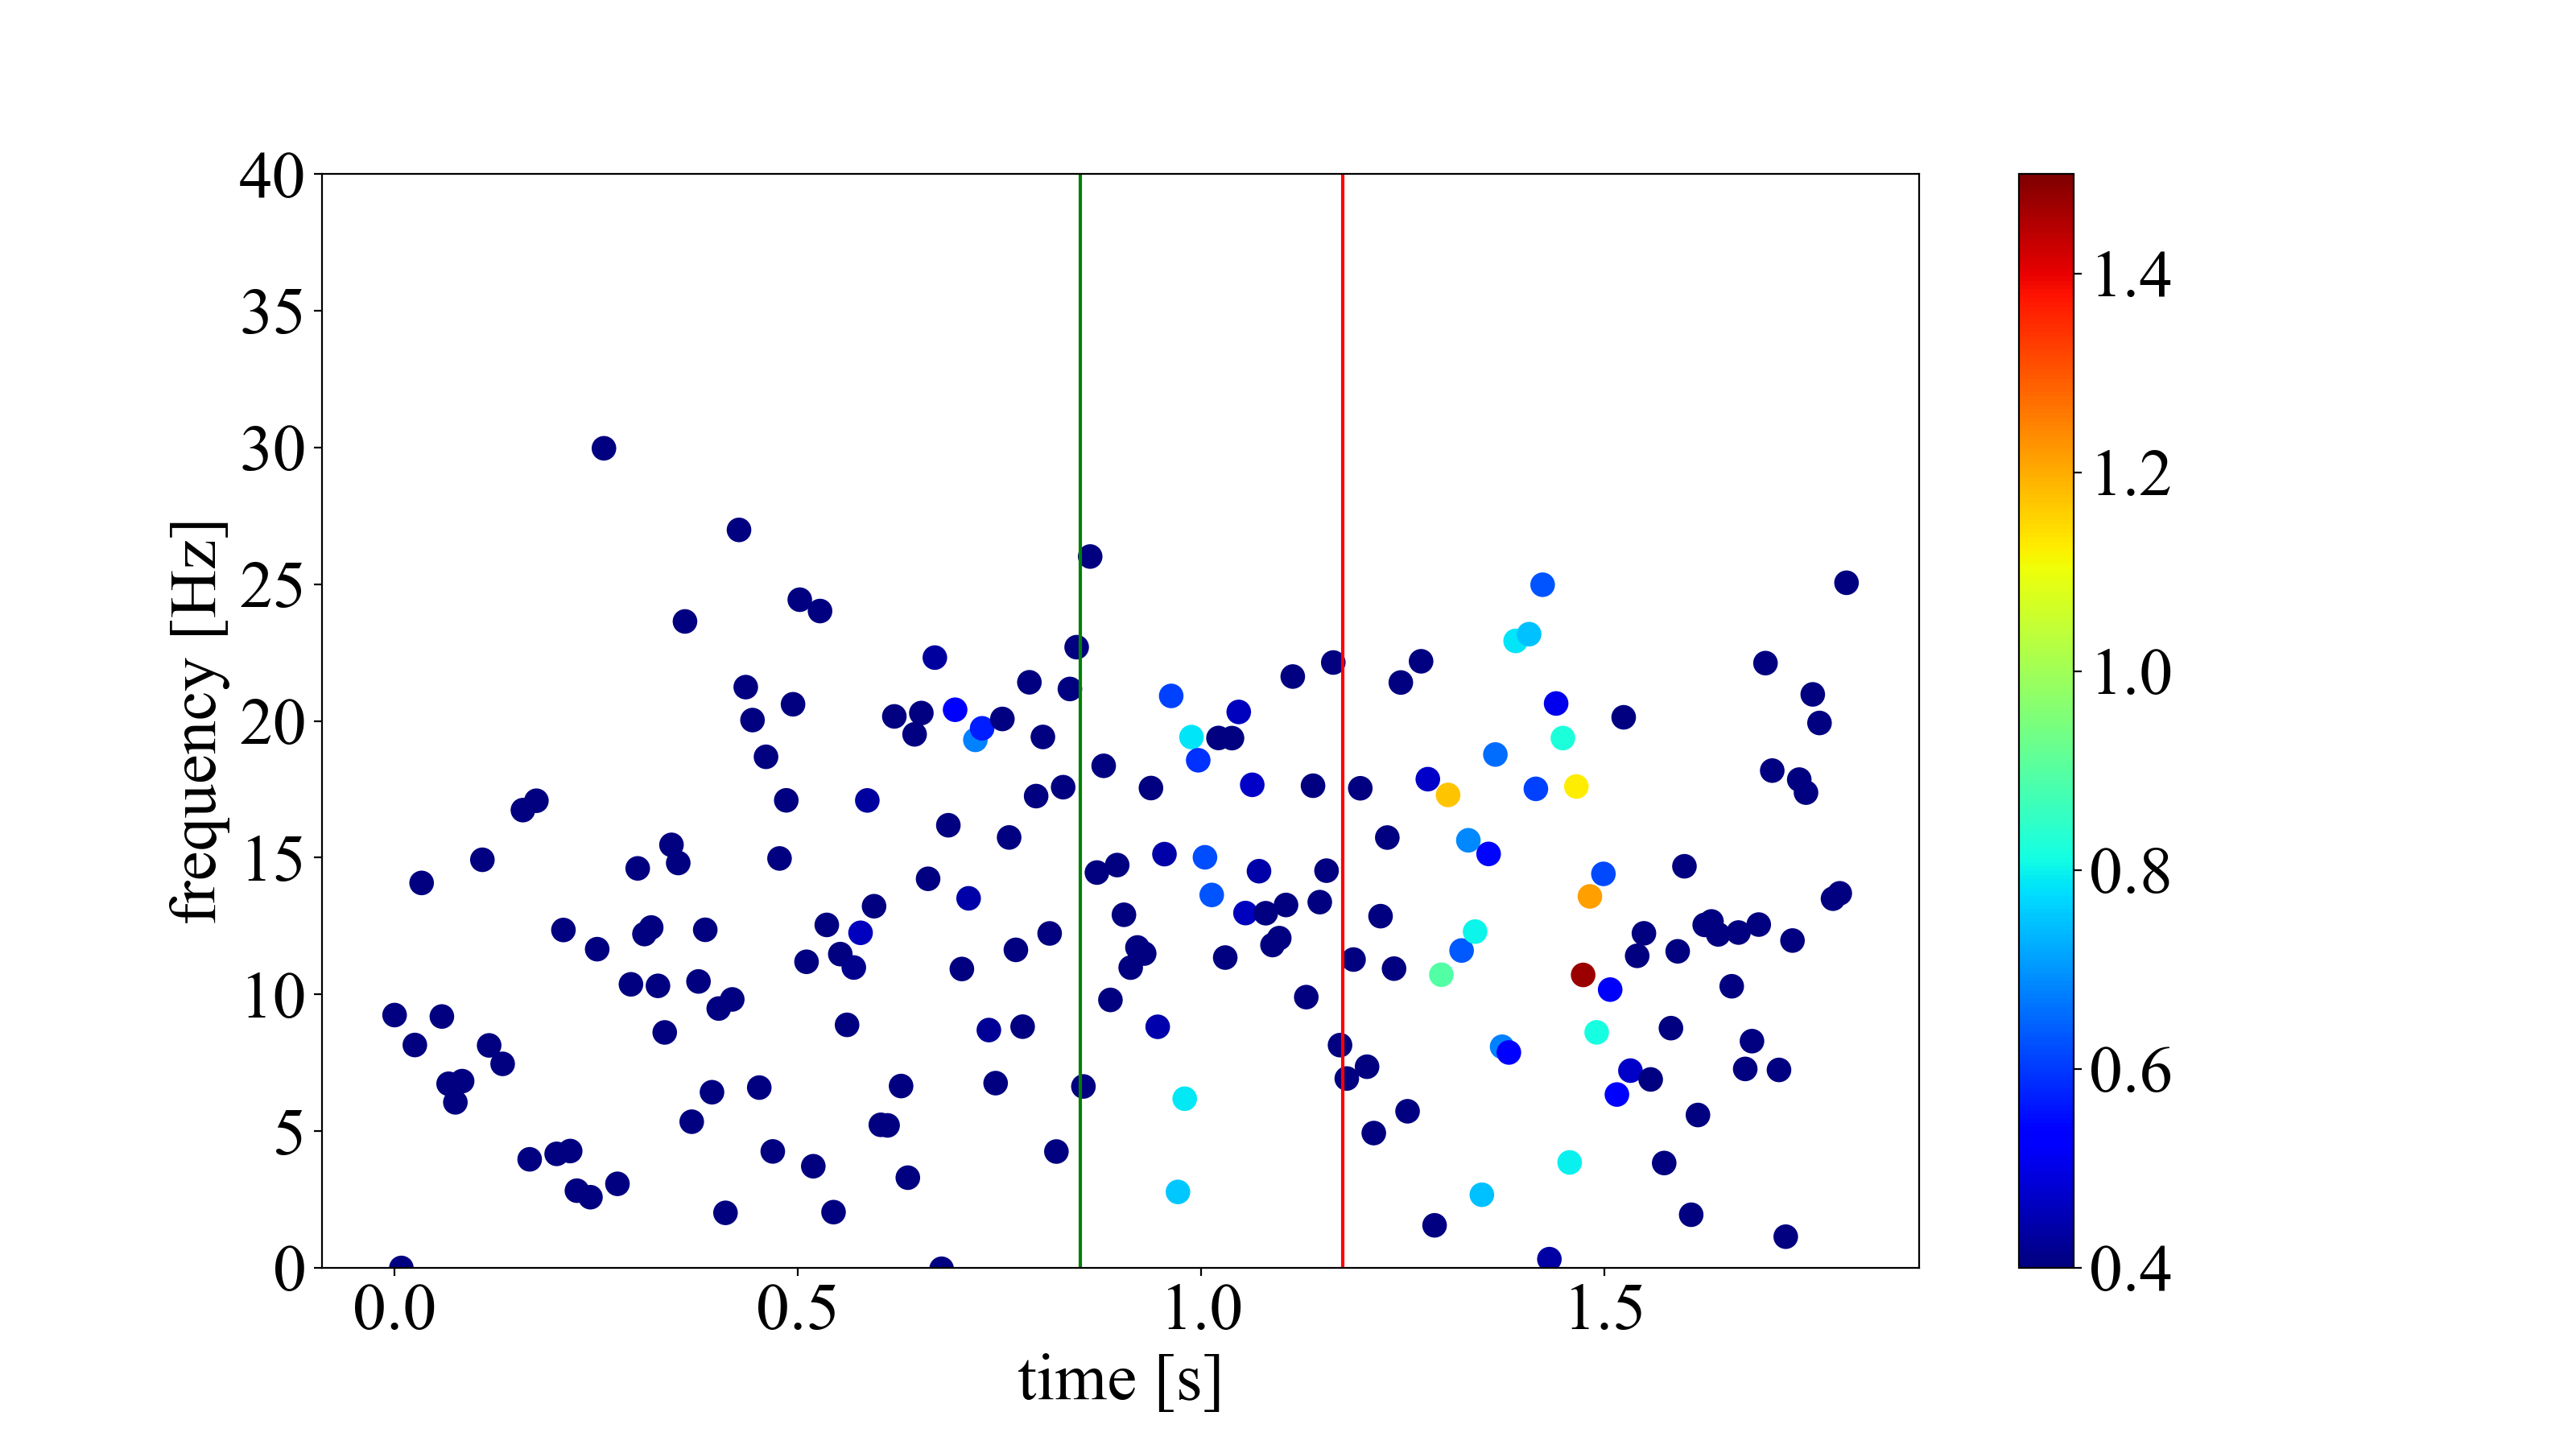
\includegraphics[width=8cm]{./images/straight_data/neck/IMF1.png}
                    % \caption{ストレート弾道で頸部モーションIMF1}
                    (a)
                    \label{straight neck imf1}
                \end{center}
            \end{minipage}

            \begin{minipage}{0.5\hsize}
                \begin{center}
                    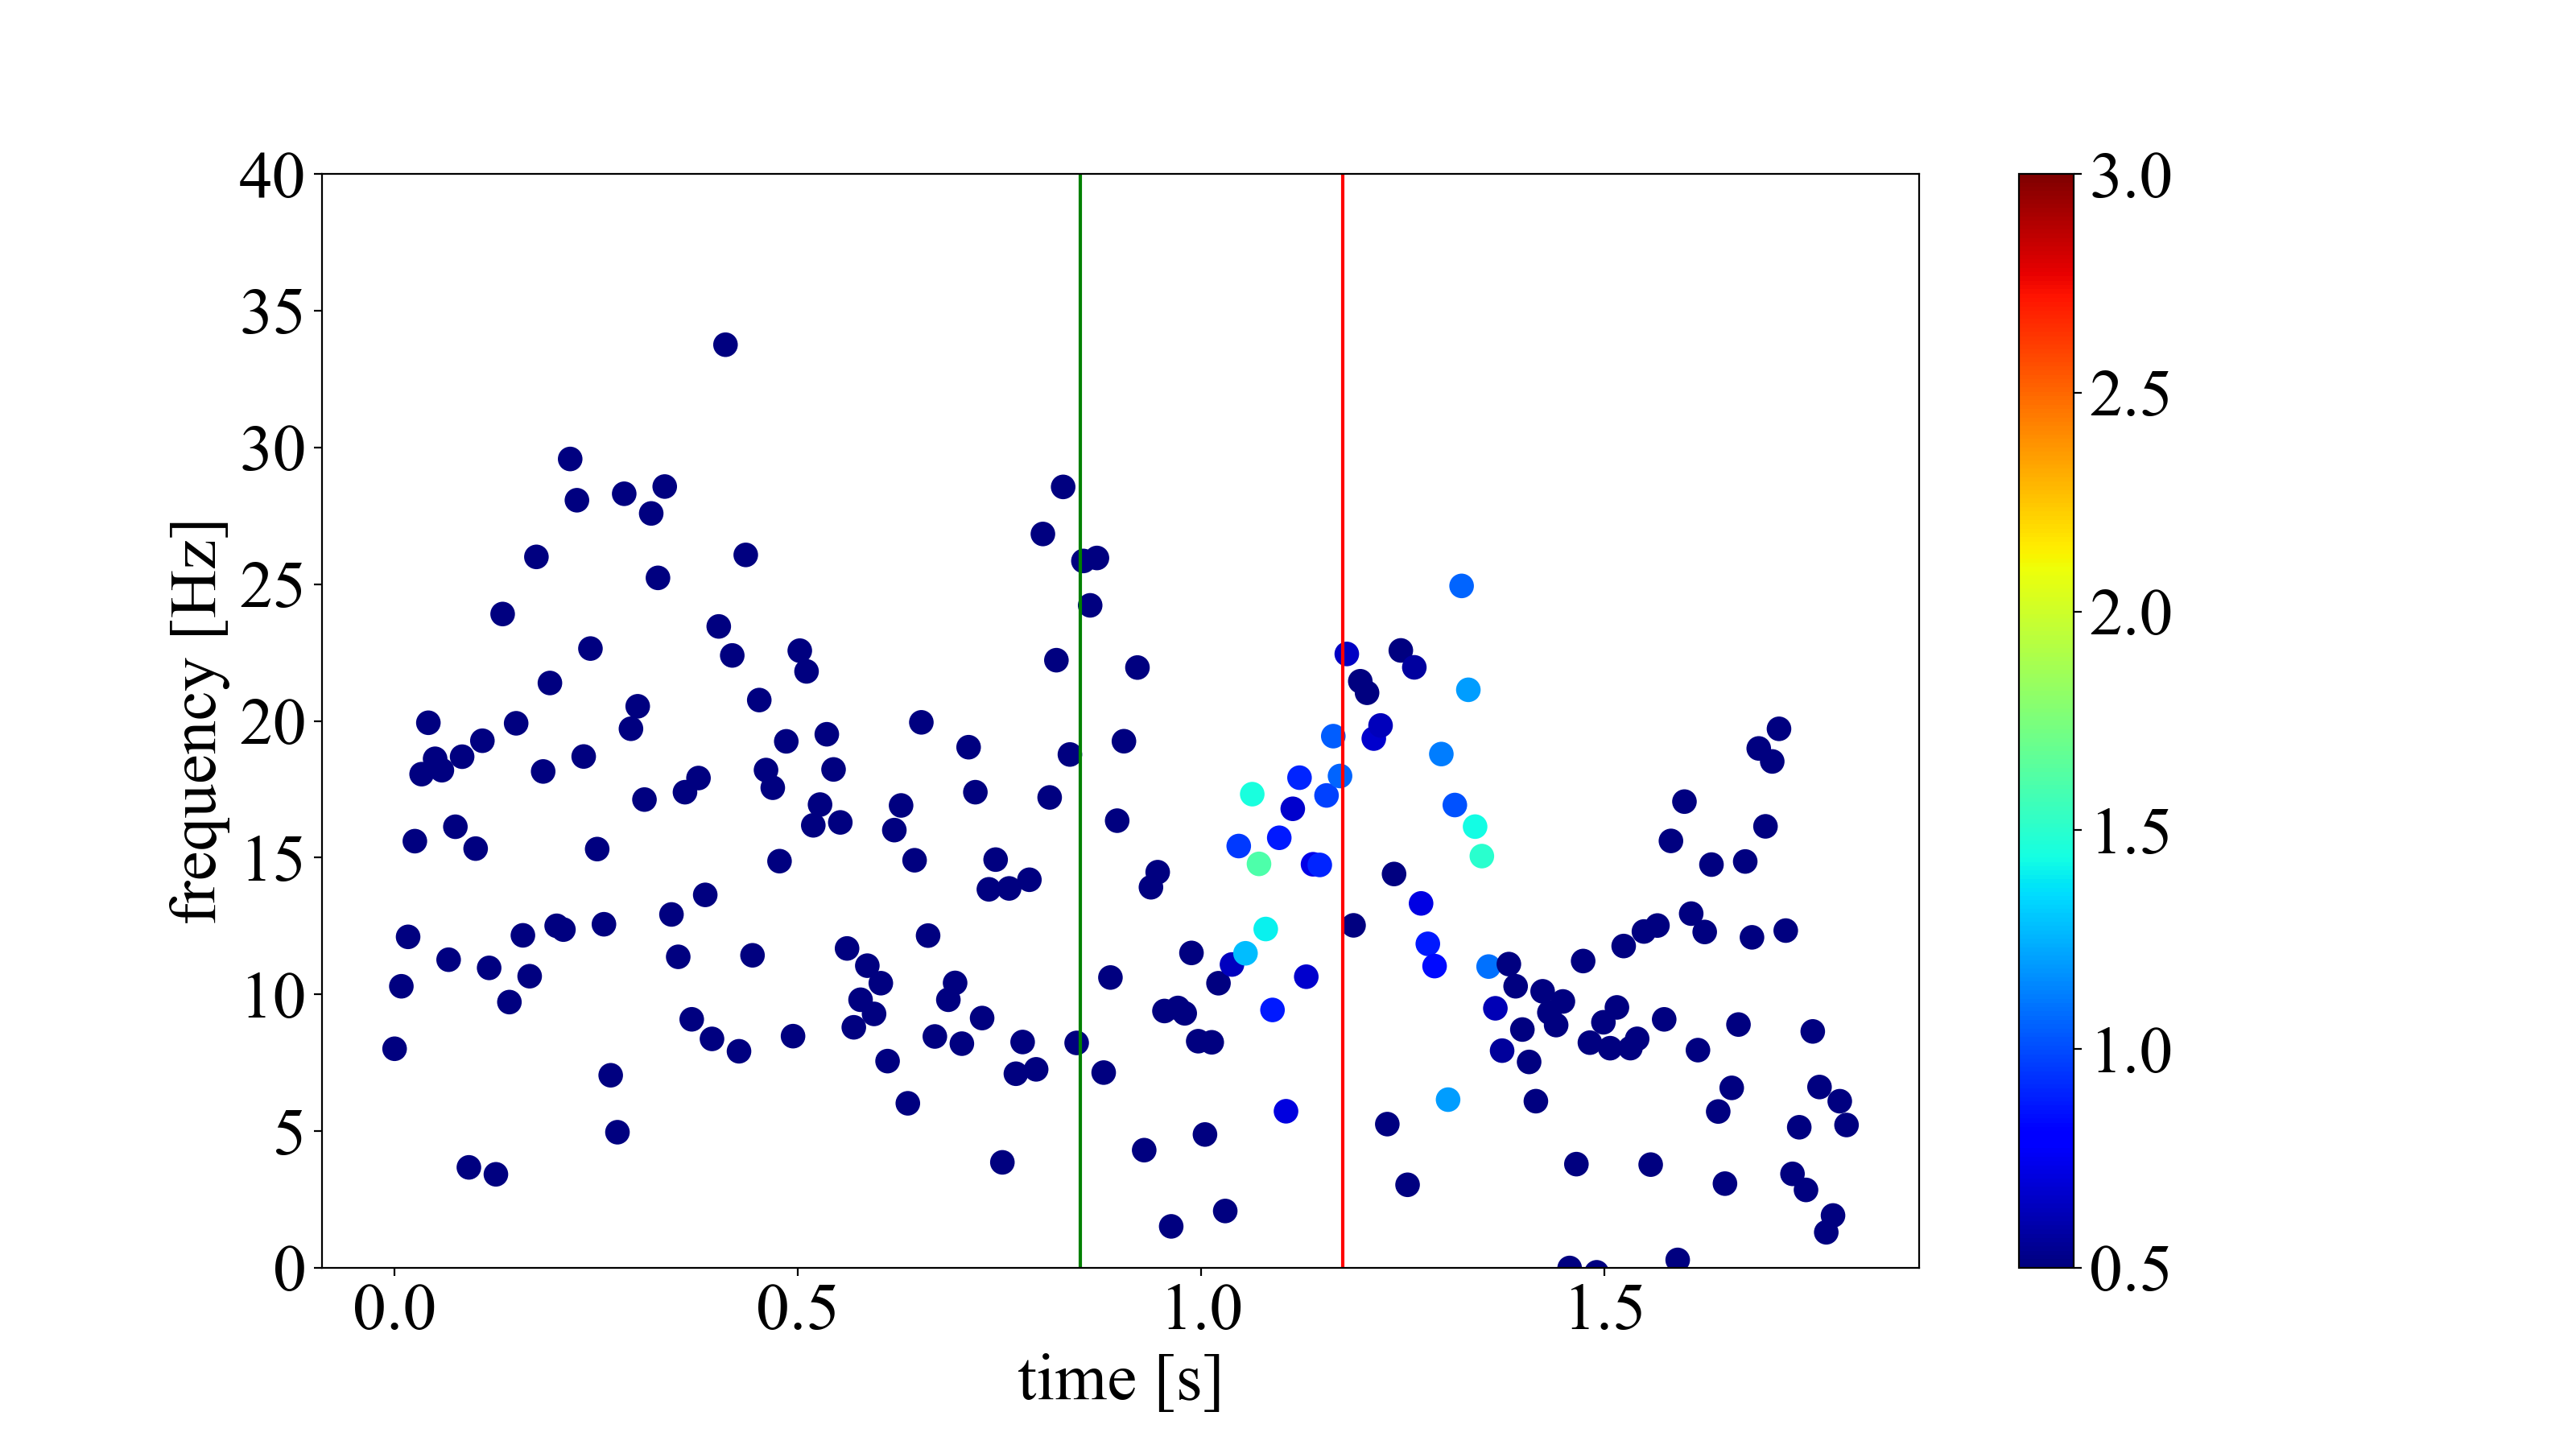
\includegraphics[width=8cm]{./images/straight_data/left_leg/IMF1.png}
                    % \caption{ストレート弾道で左膝モーションIMF1}
                    (b)
                    \label{straight left leg imf1}
                \end{center}
            \end{minipage}
        \end{tabular}
    \end{center}
\end{figure}

\begin{figure}
    \begin{center}
        \begin{tabular}{c}
            \begin{minipage}{0.5\hsize}
                \begin{center}
                    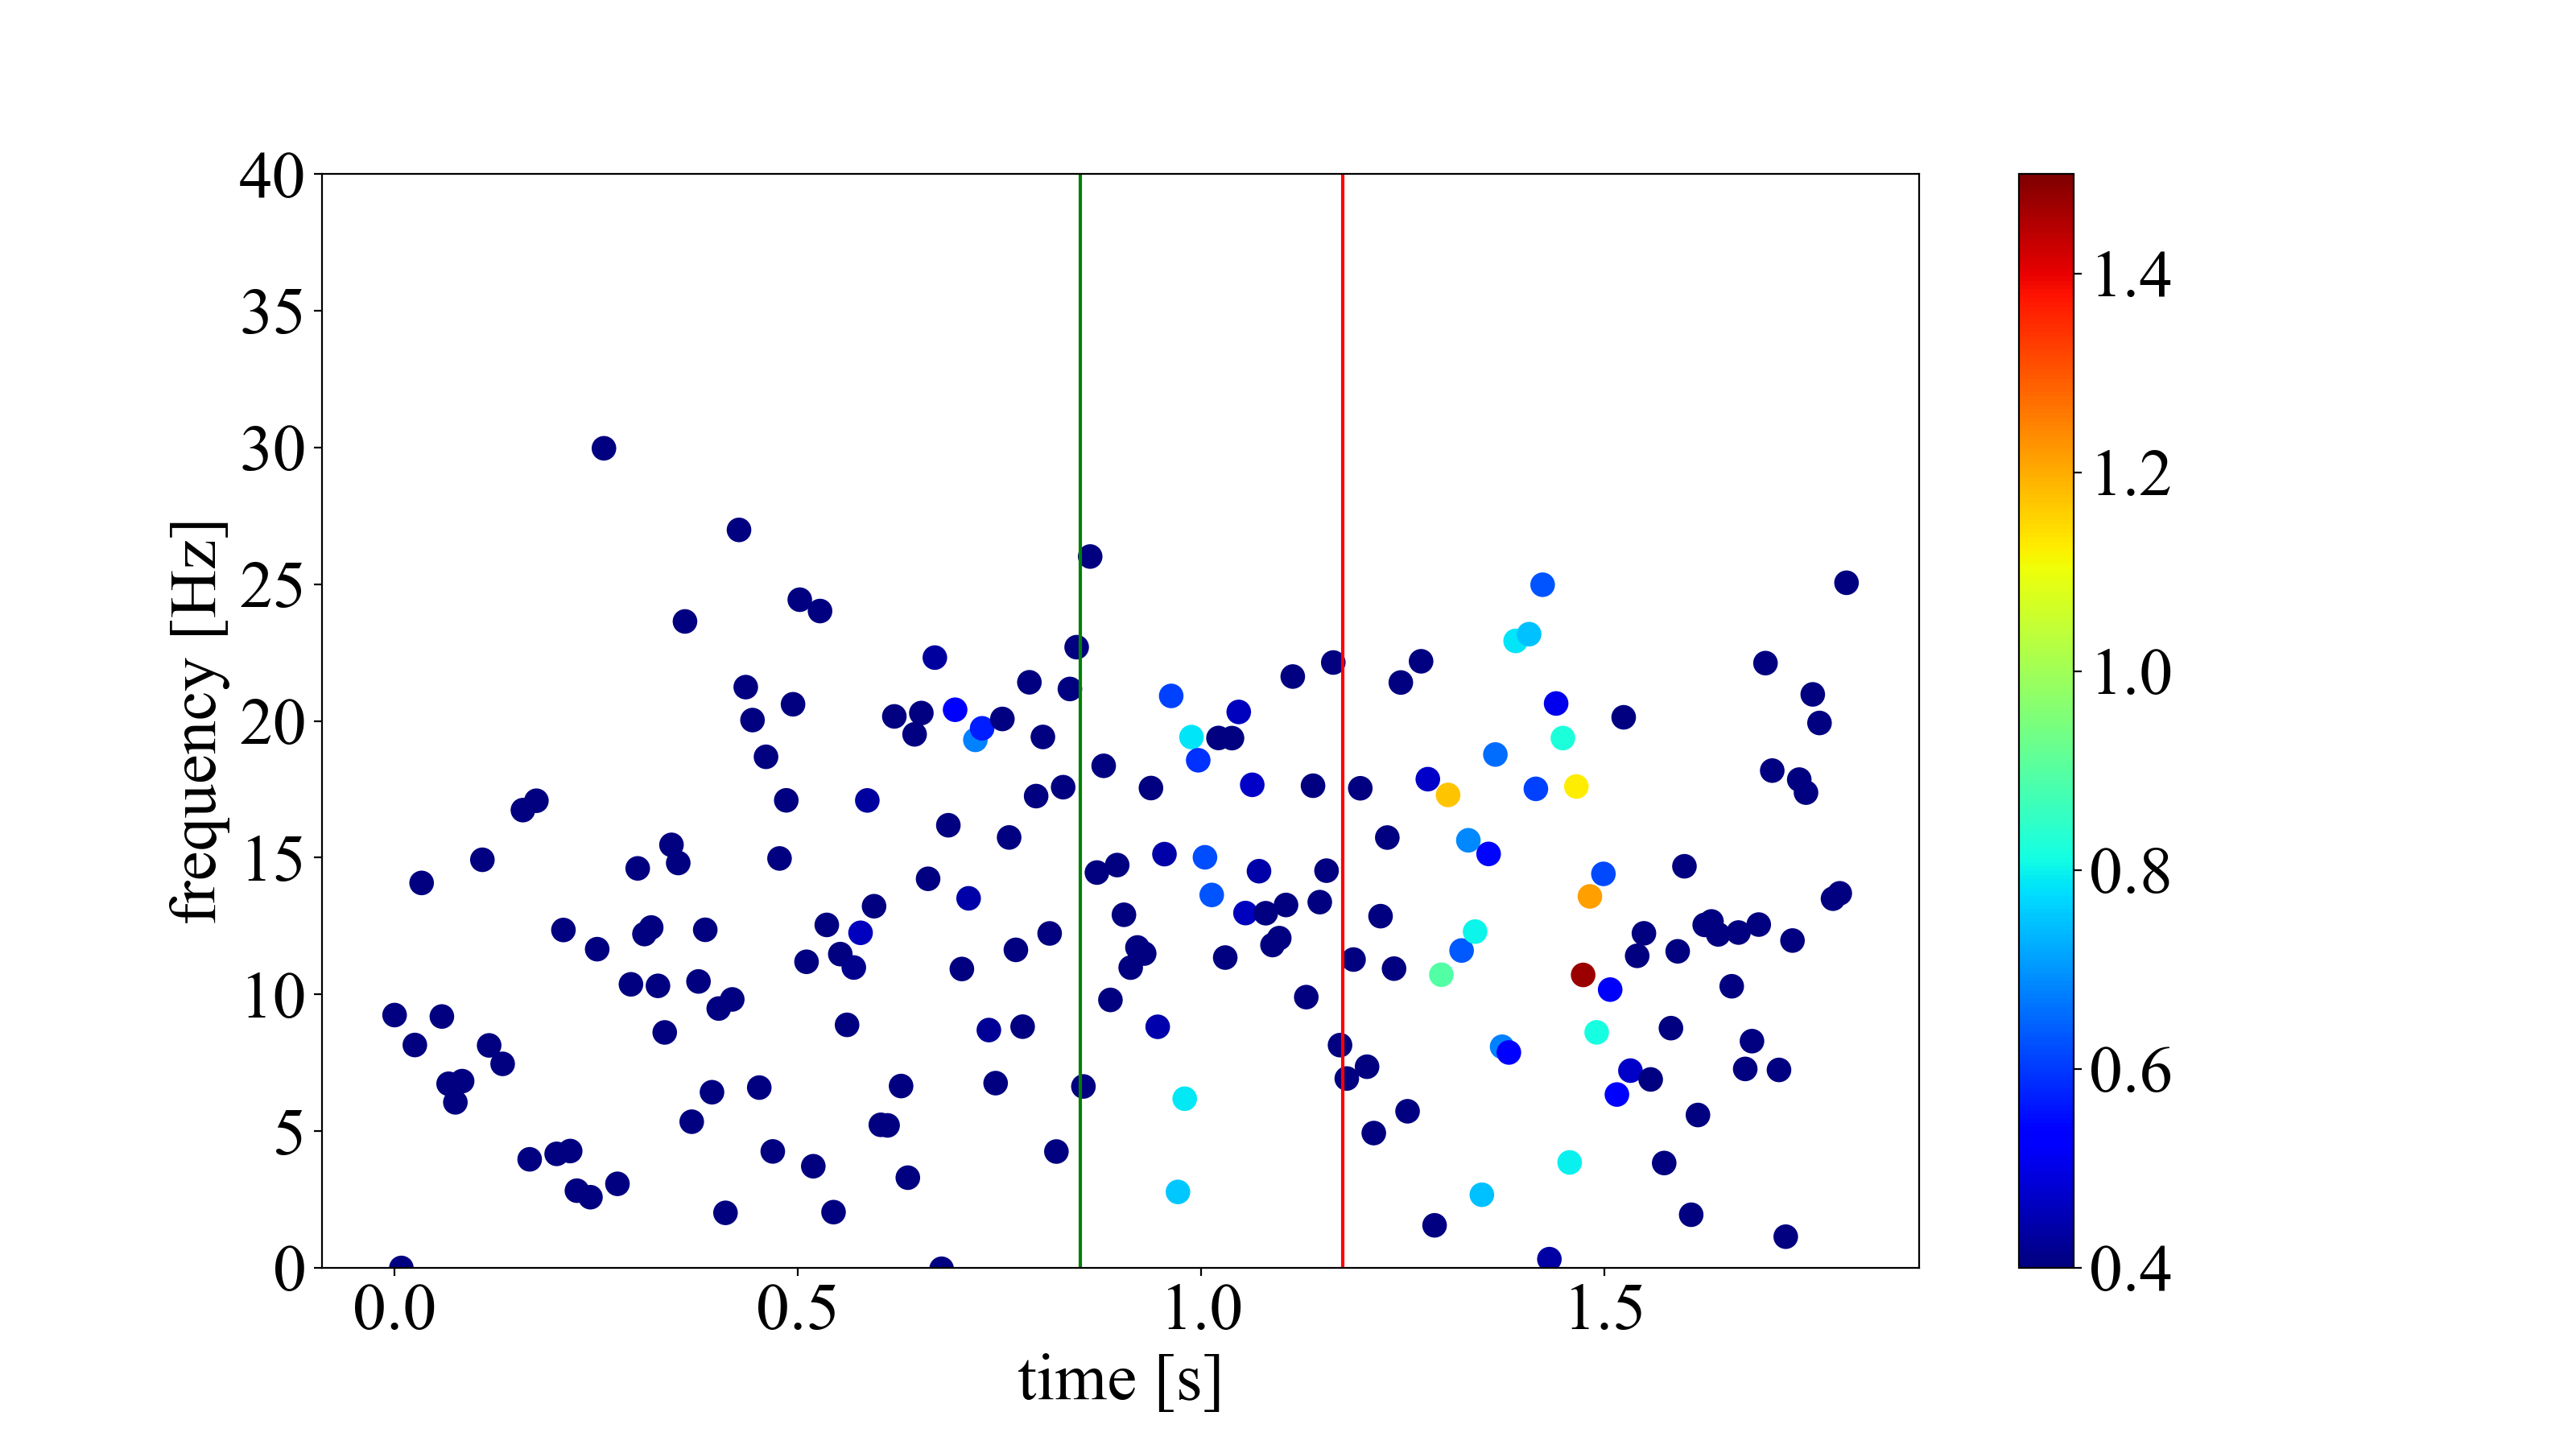
\includegraphics[width=8cm]{./images/straight_data/neck/IMF1.png}
                    % \caption{スライス弾道で頸部モーションIMF1}
                    (c)
                    \label{slice neck imf1}
                \end{center}
            \end{minipage}

            \begin{minipage}{0.5\hsize}
                \begin{center}
                    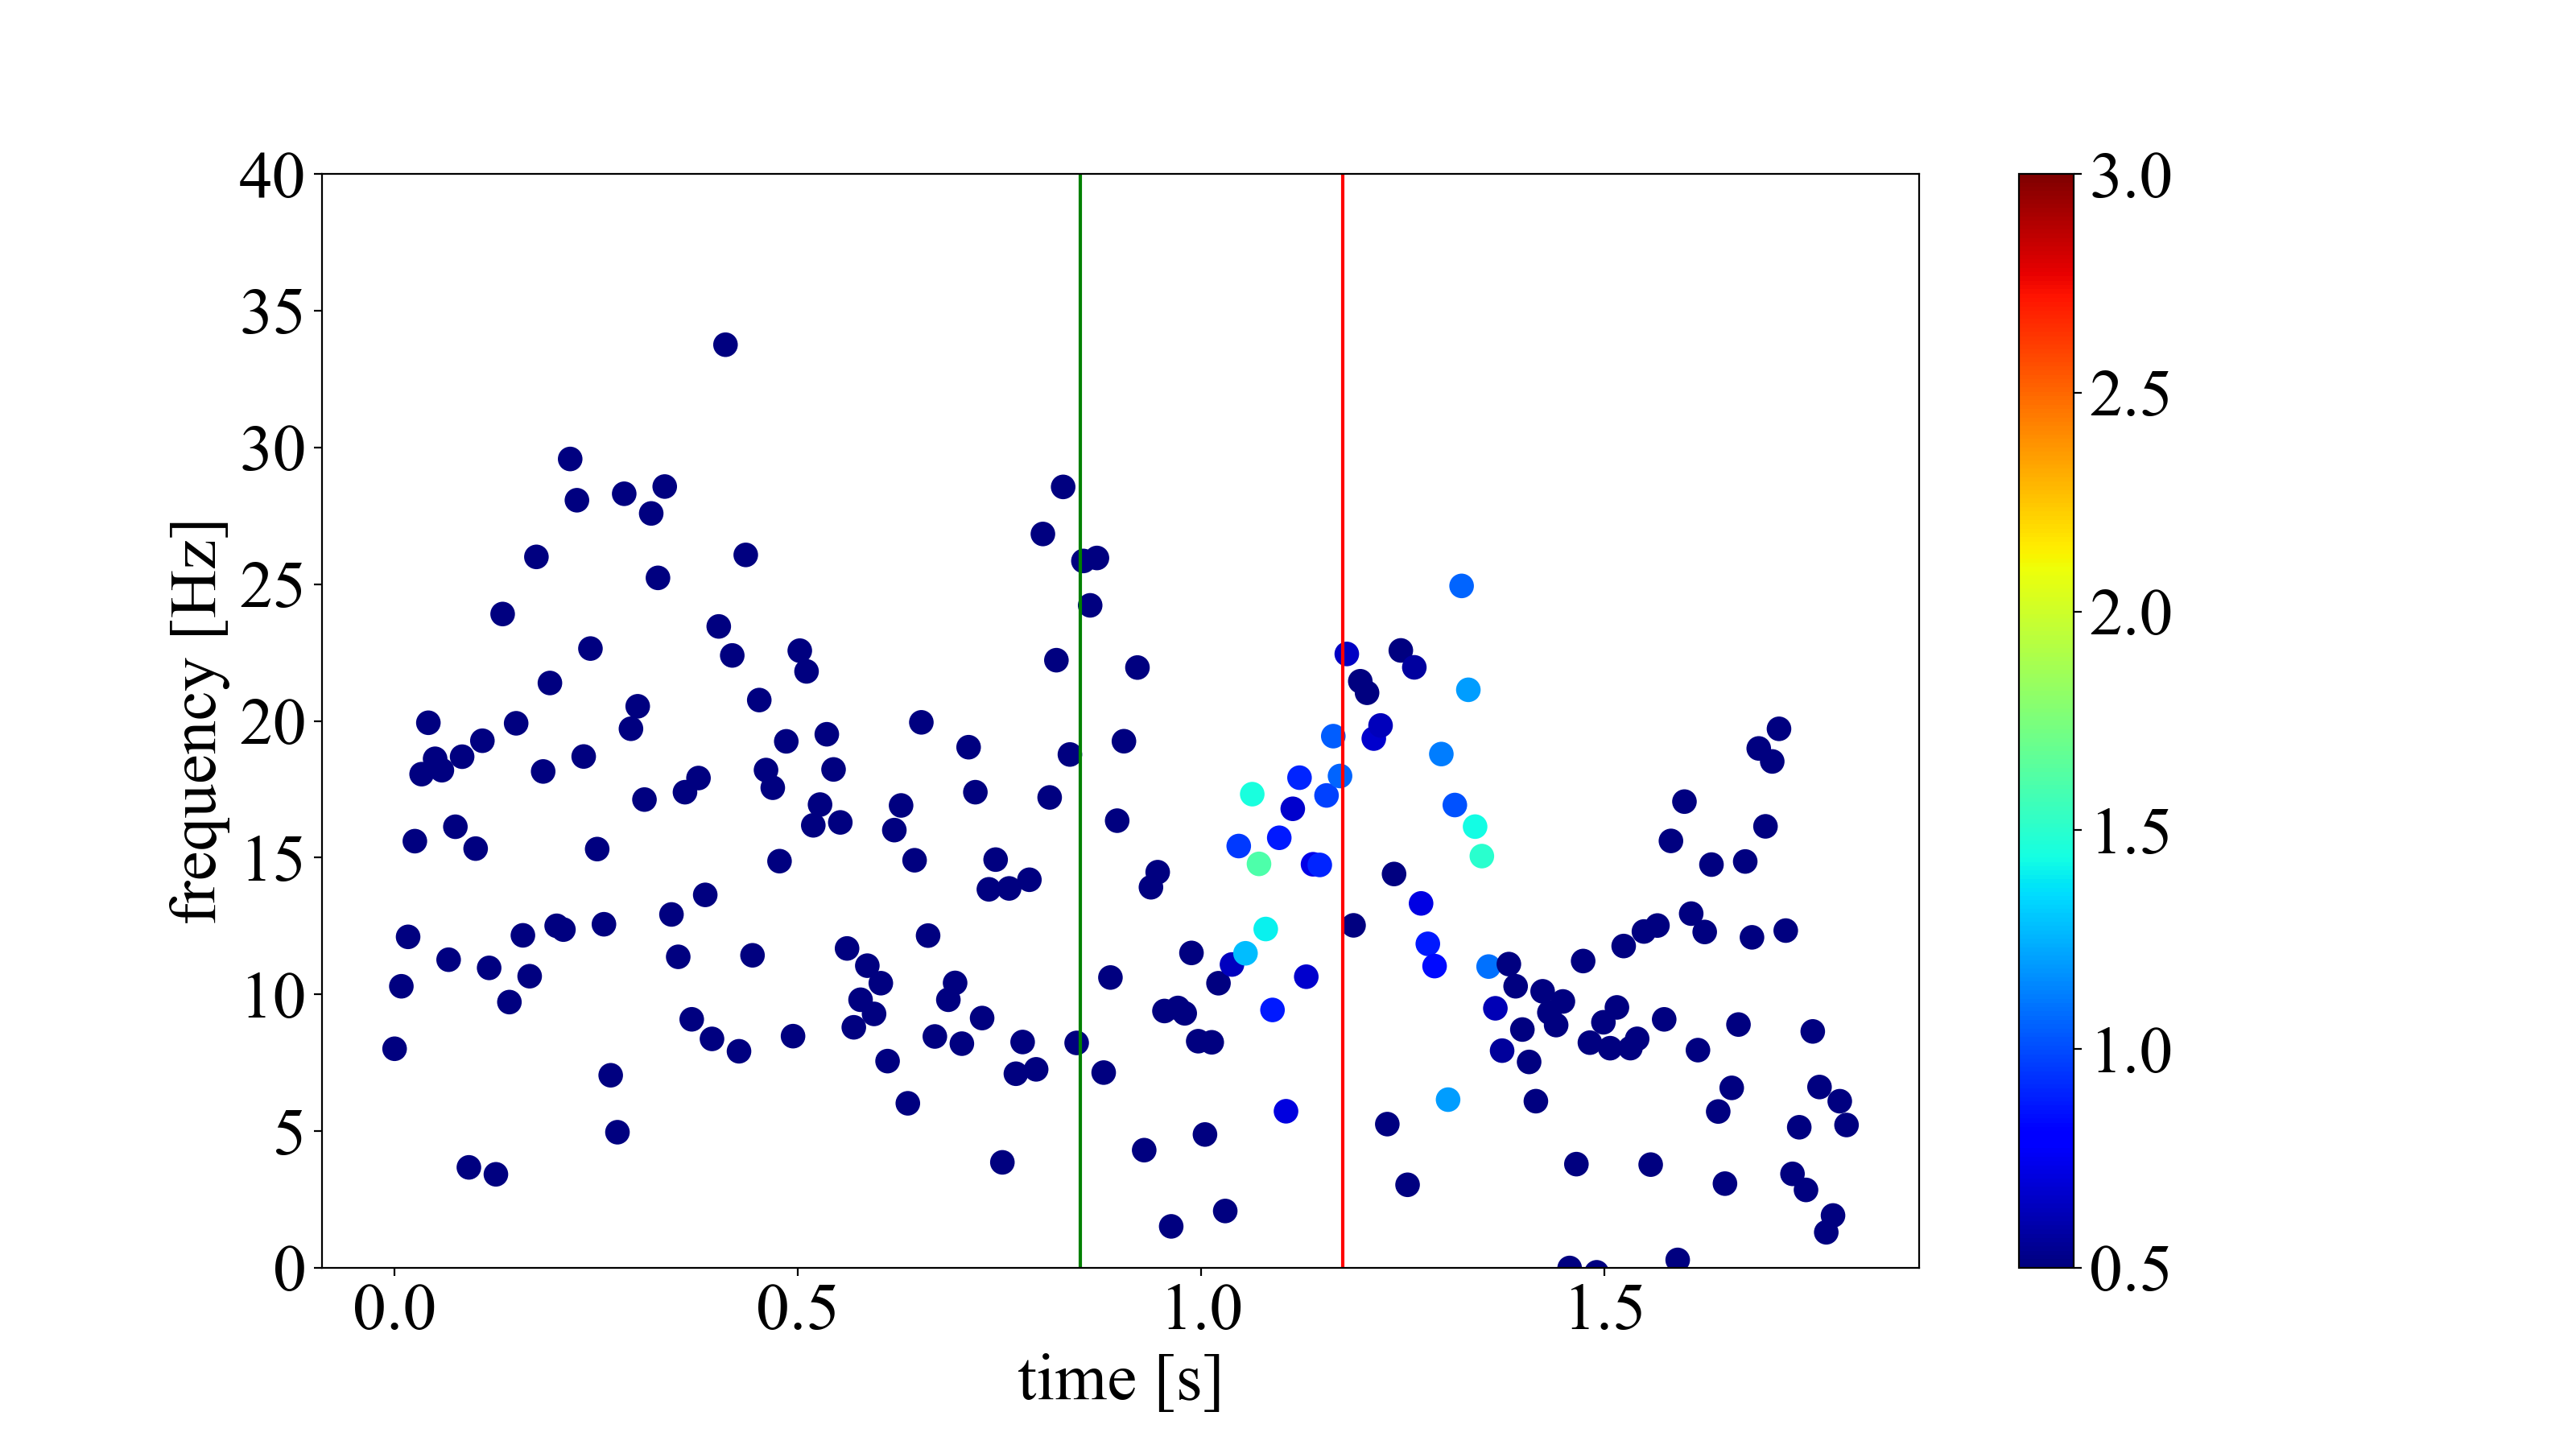
\includegraphics[width=8cm]{./images/straight_data/left_leg/IMF1.png}
                    % \caption{スライス弾道で左膝モーションIMF1}
                    (d)
                    \label{slice left leg imf1}
                \end{center}
            \end{minipage}
        \end{tabular}
    \end{center}
    \caption{ストレート弾道,スライス弾道に飛球した頸部,左膝モーションのゴルフスイングモーションスペクトル.(a)はストレート弾道で頸部モーションIMF1.(b)はストレート弾道で左膝モーションIMF1.(c)はスライス弾道で頸部モーションIMF1.(d)はスライス弾道で左膝モーションIMF1.}
    \label{imf1}
\end{figure}

被験者のドライバーショットを数値化し,ストレート弾道,ヘッドアップ動作をしたスライス弾道,身体が開く動作をしたスライス弾道の3つに分類し,各分類毎ヒルベルト・ファン変換を適用させ,瞬時周波数と瞬時振幅を計算した.
ゆえに,図\ref{imf1}は,ストレート弾道,スライス弾道に飛球したゴルフスイングで頸部モーション,左膝モーションのIMF1をスペクトログラムにしたものある.
図\ref{imf1}の赤線はインパクト,緑線はトップ,カラーバーは振幅(度)を示している.
emdでは高次成分から低次成分に分解されるため,


\subsection{頸部,左膝,左腿モーションのIMF4}	% 第4章 実装
\chapter{結論}
	% 第5章 結論
% acknowlegments.tex -- 謝辞
\theacknowledgments 本テンプレートは,以前,塙先生や生野先生をはじめとす
る先生方が作成管理していた東京工科大学の論文用テンプレートを参考させて頂
きました.先のテンプレートがなければ,本テンプレートも存在しなかったといっ
ても過言ではありません.この場を借りて感謝の意を表します.また,テンプレー
トを作成し公開したいという申し出に快く賛成・協力してくださった星先生,大
学院課の早川さんにも大変感謝しています.そして,テンプレートを作成に関わっ
たすべての人にも感謝します.本当にありがとうございました.(平成21年
G2108021 品田良太 作成)
		% 謝辞
\bibliographystyle{junsrt}
\bibliography{mybib} % 参考文献
%
% 自分の名前の下に下線を引いても良いかもしれません
%

\begin{theachievement}{99}
  \bibitem{EC2015} 岡田昌浩, 井上亮文, 星徹, ``投映面の特性を3DCGに反映させるシステムSUNDIALの色認識機能への拡張'', 情報処理学会研究報告, Vol.2015-EC-35, No.16, pp.1-7, 2015.
  \bibitem{NERU} 松尾豊, ``なぜ私たちはいつも締め切りに追われるのか'', \url{http://ymatsuo.com/papers/neru.pdf}, 2015年6月閲覧.
\end{theachievement}
 % 業績
% appendix.tex -- 付録
\appendix
\chapter{ソースコード}
\section{CONTENT}
リストファイルを\pgref{pg:CONTENT}に示す.

\lstinputlisting[caption=CONTENT,
label=pg:CONTENT]{00CONTENT}
	% 付録



\end{document}
